\documentclass[journal,12pt,twocolumn]{IEEEtran}

\usepackage{setspace}
\usepackage{gensymb}
\singlespacing
\usepackage[cmex10]{amsmath}
\usepackage{amsthm}
\usepackage{mathrsfs}
\usepackage{enumitem}
\usepackage{mathtools}
\usepackage[breaklinks=true]{hyperref}
\usepackage{graphicx}

\DeclareMathOperator*{\Res}{Res}

\renewcommand\thesection{\arabic{section}}
\renewcommand\thesubsection{\thesection.\arabic{subsection}}

\begin{document}

\newcommand{\question}{\noindent \textbf{Question: }}
\newcommand{\solution}{\noindent \textbf{Solution: }}
\newcommand{\myvec}[1]{\ensuremath{\begin{pmatrix}#1\end{pmatrix}}}

\let\vec\mathbf

\title{ASSIGNMENT-1}
\author{CS21BTECH11024 - Varshini  Jonnala}	
\maketitle
\bigskip
\section*{ICSE 10 2018 - Problem 7(c)}

\question $\vec{A}\myvec{2\\5}$, $\vec{B}\myvec{-1\\2}, \vec{C}\myvec{5\\8}$ are the vertices of the triangle $\vec{ABC}$, $\vec{`M'}$ is a point on $\vec{AB}$ such that $AM:MB = 1:2$. Find the co-ordinates of $\vec{`M'}$. Hence find the equation of line passing through the points $\vec{C}$ and $\vec{M}$.
\newline \newline
\solution According to the question, $\vec{M}$ is a point on the side $\vec{AB}$ such that $$AM : MB = 1 : 2$$
 When the line segment $\vec{AB}$, where the points are $\vec{A}=\myvec{x1\\y1}, \vec{B}=\myvec{x2\\y2}$, is divided internally by $\vec{C}$ in the ratio $m:n$, from Section formula,
 we get the Coordinates of point $\vec{C}$ as,
\begin{align} 
\vec{C} = \myvec{\frac{mx2+nx1}{m+n}\\\\ \frac{my2+ny1}{m+n}},\label{1}
\end{align}
From given data, Using \eqref{1} in finding $\vec{M}$, we get
\begin{align}
    \vec{M} &= \myvec{\frac{-1+4}{1+2}\\\\ \frac{2+10}{1+2}}\\  \label{3}
   &= \myvec{1\\4}
\end{align}\newline
The equation of the line joining two points \myvec{a\\b} and \myvec{c\\d} is 
\begin{align}
    \myvec{y-b} = {\myvec{\frac{d-b}{c-a}}}\myvec{x-a} \label{5}
\end{align}
Here, the equation of the line joining points $\vec{C}\myvec{5\\8}$ and $\vec{M}\myvec{1\\4}$ will be
\begin{align}
    \myvec{y-4} = \myvec{\frac{8-4}{5-1}}\myvec{x-1} \label{6}
\end{align}
Simplified, we get the equation
\begin{align}
    \myvec{1 & - 1}\vec{x} &= -3 
\end{align}
 which can also be represented as 
 \begin{align}
     x-y+3=0
 \end{align}
\subsection*{But, However,} On using \eqref{5}, we get
\newline
\begin{enumerate}
    \item The equation of the line joining $\vec{A}\myvec{2\\5}, \vec{B}\myvec{-1\\2}$ as $\myvec{1 & - 1}\vec{x} = -3$ and 
    \newline
    \item The equation of the line joining $\vec{B}\myvec{-1\\2}, \vec{C}\myvec{5\\8}$ as $\myvec{1 & - 1}\vec{x}=-3$ too.\newline
\end{enumerate}
 This implies that $\vec{A,B,C}$ points are `collinear' and lie on the line $\myvec{1 & - 1}\vec{x} = -3$ (or) $x-y+3=0$ and Hence, given points $\vec{A,B,C}$ don't form a triangle.
\newline\newline
Verified by plotting the graph of $\vec{A,B,C}$ and $\vec{M}$ points :
 
\begin{figure}[ht!]
\centering
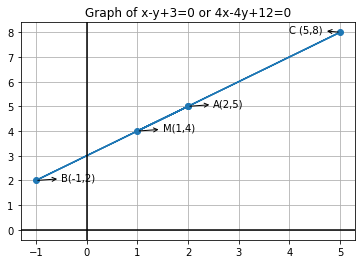
\includegraphics[width=\columnwidth]{prv1.png}
\end{figure}
 
\end{document}

